\documentclass{standalone}
\usepackage{tikz}

\usetikzlibrary{calc}


\begin{document}

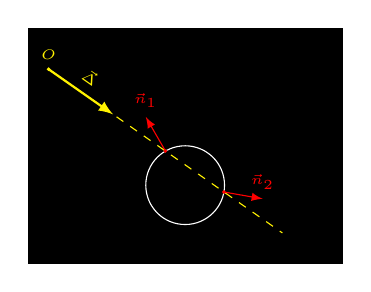
\begin{tikzpicture}
  \path[fill=black] (-2,-1) rectangle (2,2);
  \draw[white] (0,0) circle [radius=0.5cm];

  \coordinate (P1) at (120:0.5);
  \coordinate (P2) at (-10:0.5);
  \coordinate (O) at ($ (P1) ! -2 ! (P2) $);

  \path[fill=red] (P1) circle [radius=0.025cm];
  \path[fill=red] (P2) circle [radius=0.025cm];

  \draw[dashed,yellow] (O) -- ($ (P1) ! 2 ! (P2) $);
  \path[fill=yellow] (O) circle [radius=0.025cm] node[above,font=\tiny,yellow] {$O$};
  \draw[-latex,thick,yellow] (O) -- ($ (O) ! 1cm ! (P1) $) node[midway,above,sloped,font=\tiny] {$\vec\Delta$};

  \draw[-latex,red] (P1) -- ($ (0,0) ! 2 ! (P1) $) node[above,font=\tiny] {$\vec n_1$};
  \draw[-latex,red] (P2) -- ($ (0,0) ! 2 ! (P2) $) node[above,font=\tiny] {$\vec n_2$};
\end{tikzpicture}

\end{document}